\documentclass{ds-report}
\assignment{JAVA RMI} % Set to `Java RMI`, `Java EE` or `Google App Engine`.
\authorOne{Dries Janse} % Name of first team partner.
\studentnumberOne{r0627054} % Student number of first team partner.
\authorTwo{Steven Ghekiere} % Name of second team partner.
\studentnumberTwo{r0626062}  % Student number of second team partner.


\begin{document}
	\maketitle

	\paragraph{1. How would a client complete one full cycle of the booking process, for both a successful and
failed case? Base yourself on the example scenarios of the assignment. Create sequence drawings to illustrate this.} \mbox{}\\\\
The complete cycle of the booking process, based on the example scenarios as given in the assignment are visualized in Figure \ref{fig:sequence_diagram}.

	
	\paragraph{2. When do classes need to be serializable? You may illustrate this with an example class.} \mbox{}\\\\
When a Java class implements the java.io.Serializable interface, an instance of this class can be passed as a result or an argument in Java RMI. These instances, just as all primitive types, are copied and passed by value. This means that the receiver creates a copy of the object. On this copied object, methods can be invoked but this will only change the local object. The state of the local object can be different from the state of the original object of the sender. \\\\
Classes need to be serializable when the value of the object of such a class is needed. The users, of these classes, are not allowed to modify the original objects. In our project, we made the following classes explicitly serializable:
\begin{itemize}
	\item CarType 
	\item ReservationConstraints 
	\item Quote
	\item Reservation (subclass of Quote)
\end{itemize}
The following classes, used in our project, are already serializable: String, Date, HashSet, ArrayList and HashMap.\\\\
To illustrate this with an example: the client class can request a list of available car types. It requests this list by invoking the getAvailableCarTypes method on the remote object reference of his reservation session. This will return an ArrayList of car types. These types are passed by value, this is done because the client classes are not allowed to change the information of the actual car types.
\clearpage
	\paragraph{3. When do classes need to be remotely accessible (Remote)? You may illustrate this with an example
class.} \mbox{}\\\\
Instances of classes which are remotely accessible (implement the java.rmi.Remote interface) are passed by remote object reference. The object which receives this remote object reference can make RMI calls on this remote object. Because no copy is made of the object, the original object of the sender is modified. All the classes, which have to be remote, have to implement an interface specifying all the methods which can be invoked remotely. This interface directly extends the java.rmi.Remote interface and is implemented by the remote class.\\\\
In our project the following remote interfaces are created:
\begin{itemize}
	\item INamingService
	\item ICarRentalCompany
	\item IManagerSession
	\item IReservationSession
	\item IRentalAgency
\end{itemize} 
The INamingService is a remote interface used for registering, unregistering and requesting car rental companies to the naming service. The ICarRentalCompany is a remote interface used for requesting and manipulating car rental company data. It is used by both the reservation and manager session. The IReservationSession is a remote interface used for creating, requesting, confirming quotes and requesting car types. The IManagerSession is a remote interface used for registering/unregistering car rental companies and requesting general information such as the number of reservations, best customers and popular car types. The IRentalAgency is a remote interface used for creating and closing sessions.

	\paragraph{4. What data has to be transmitted between client and server and back when requesting the number of reservations of a specific renter?} \mbox{}\\\\
When calling the getNumberOfReservationsByRenter method in the client class, two parameters are required: the name of the client of which the client wishes to receive the information and a remote object reference of the IManagerSession. This IManagerSession is stored on the RentalAgency server. On this manager session reference the client will invoke the remote getNumberOfReservations method, which needs the name of the client. This client name string will be marshalled and send by value to the RentalAgency server where the manager session is stored. It will first request all the car rental companies references at the naming service. The naming service server will return all the car rental company references it contains, to the rental agency server. The manager session does this by invoking the getCarRentalCompanies method on the naming service reference.
Thereafter, the getReservationsByRenter method is called by the manager session on each of the car rental companies references, to calculate the total amount of reservations. Finally the manager session stored on the rental agency server will return the total amount of reservations of the renter back to the client by value.   

\clearpage
	\paragraph{5. What is the reasoning behind your distribution of remote objects over hosts? Show which hosts execute which classes, if run in a real distributed deployment (not a lab deployment where everything runs on the same machine). Create a component/deployment diagram to illustrate this: highlight where the client and server are.} \mbox{}\\\\
Figure \ref{fig:deployment_diagram} shows the deployment diagram of the application. This diagram shows how the different classes can be deployed in a real distributed deployment. The clients are: the client node and the manager node. The other nodes can be identified as different servers. These servers can all be placed on different physical machines or grouped together (multiple possibilities).

	\paragraph{6. How have you implemented the naming service, and what role does the built-in RMI registry play? Why did you take this approach?} \mbox{}\\\\
The NamingService class is used to store all the ICarRentalCompany remote object references. It does this by making use of a HashMap where the key is the name of the company and the value is the remote object reference of the car rental company. By making use of this data structure a company reference is easily accessed by its name and no duplicate companies can exist.\\\\
The NamingService class itself implements the INamingService interface. This interface extends the java.rmi.Remote interface and contains the methods to register, unregister and request remote car rental company object references.\\\\
To start the naming server, a NamingServiceApplication class is used. This class only contains a main method which creates an instance of the naming service, exports it as a remote object and binds it to the RMI registry. The car rental agency can lookup this naming service on the RMI registry.\\\\
This design is chosen because it ensures that the components are loosely coupled and have high cohesion. This design makes it possible to run the naming service on a different server than the car rental agency. The car rental agency only needs an identifier of the naming server so it can lookup the remote object reference using the RMI registry.
 

	\paragraph{7. Which approach did you take to achieve life cycle management of sessions? Indicate why you picked this approach, in particular where you store the sessions.} \mbox{}\\\\
All the sessions, both the manager and reservation, are stored on the rental agency. The sessions are stored in a HashMap, with as key the name of the client and the value is equal to the session. The rental agency is responsible for creating, storing and closing sessions. When the client asks for a reservation session, the agency first tries to find an existing reservation session with a matching client name. The agency does this for reusing sessions if they where already created. If a session was already created, the agency will return this session, otherwise a new reservation session will be created and stored on the agency. The same approach is used for the manager session.\\\\
For cleaning the sessions, the client explicitly invokes the closeReservationSession method on the remote object reference of the agency as suggested in the assignment. The name of the client, which is the same name as the session, is given as an argument to the remote procedure. The rental agency searches the session with the matching name, and removes this session from the map.

\clearpage
	\paragraph{8. Why is a Java RMI application not thread-safe by default? How does your application of synchronization achieve thread-safety?} \mbox{}\\\\
A Java RMI application is not thread-safe by default because the RMI runtime makes no guarantees of the mapping of remote object invocations to theads. Method invocations on the same remote object can be executed concurrently. This is why the remote object implementation needs to make its implementation thread-safe.\\\\
To achieve synchronization in Java, there are two choices: either the synchronized tag is set on the method declaration or the synchronized tag is set on a certain data structure. The first option means that if the client calls this method, the server will never pause this method during execution. The second option, which is more fine grained, 'locks' a certain data structure for a certain amount of statements, in which this object will never be able to be changed by another process that wishes to do so.\\\\
We made use of synchronization in the application in the following classes:
\begin{itemize}
	\item NamingService: in both the register and unregister methods, the companies HashMap is synchronized. 
	\item CarRentalCompany: the cancelReservationSession method is synchronized.
	\item ReservationSession: the confirmQuotes method is synchronized.
	\item RentalAgency: in the createNewReservationSession, createNewManagerSession, closeManagerSession and CloseReservationSession, the sessions map is synchronized.
\end{itemize} 


	\paragraph{9. How does your solution to concurrency control affect the scalability of your design? Could synchronization become a bottleneck?} \mbox{}\\\\
All the synchronization in the project is used to achieve thread-safety. For a small agency application it does not create a bottleneck. But if the application is scaled up, there will be a bottleneck. The rental agency will become the single point of failure because this contains all the sessions which will handle the confirmation of quotes. These quotes are confirmed in a synchronized way. A possible solutions for this problem is to handle quote confirmation in a concurrent way, this can be done if the list of quotes does not contain the same companies. Also the session management can become a bottleneck for the agency because the map of sessions needs to be synchronized.

	
	\clearpage
\begin{figure}
  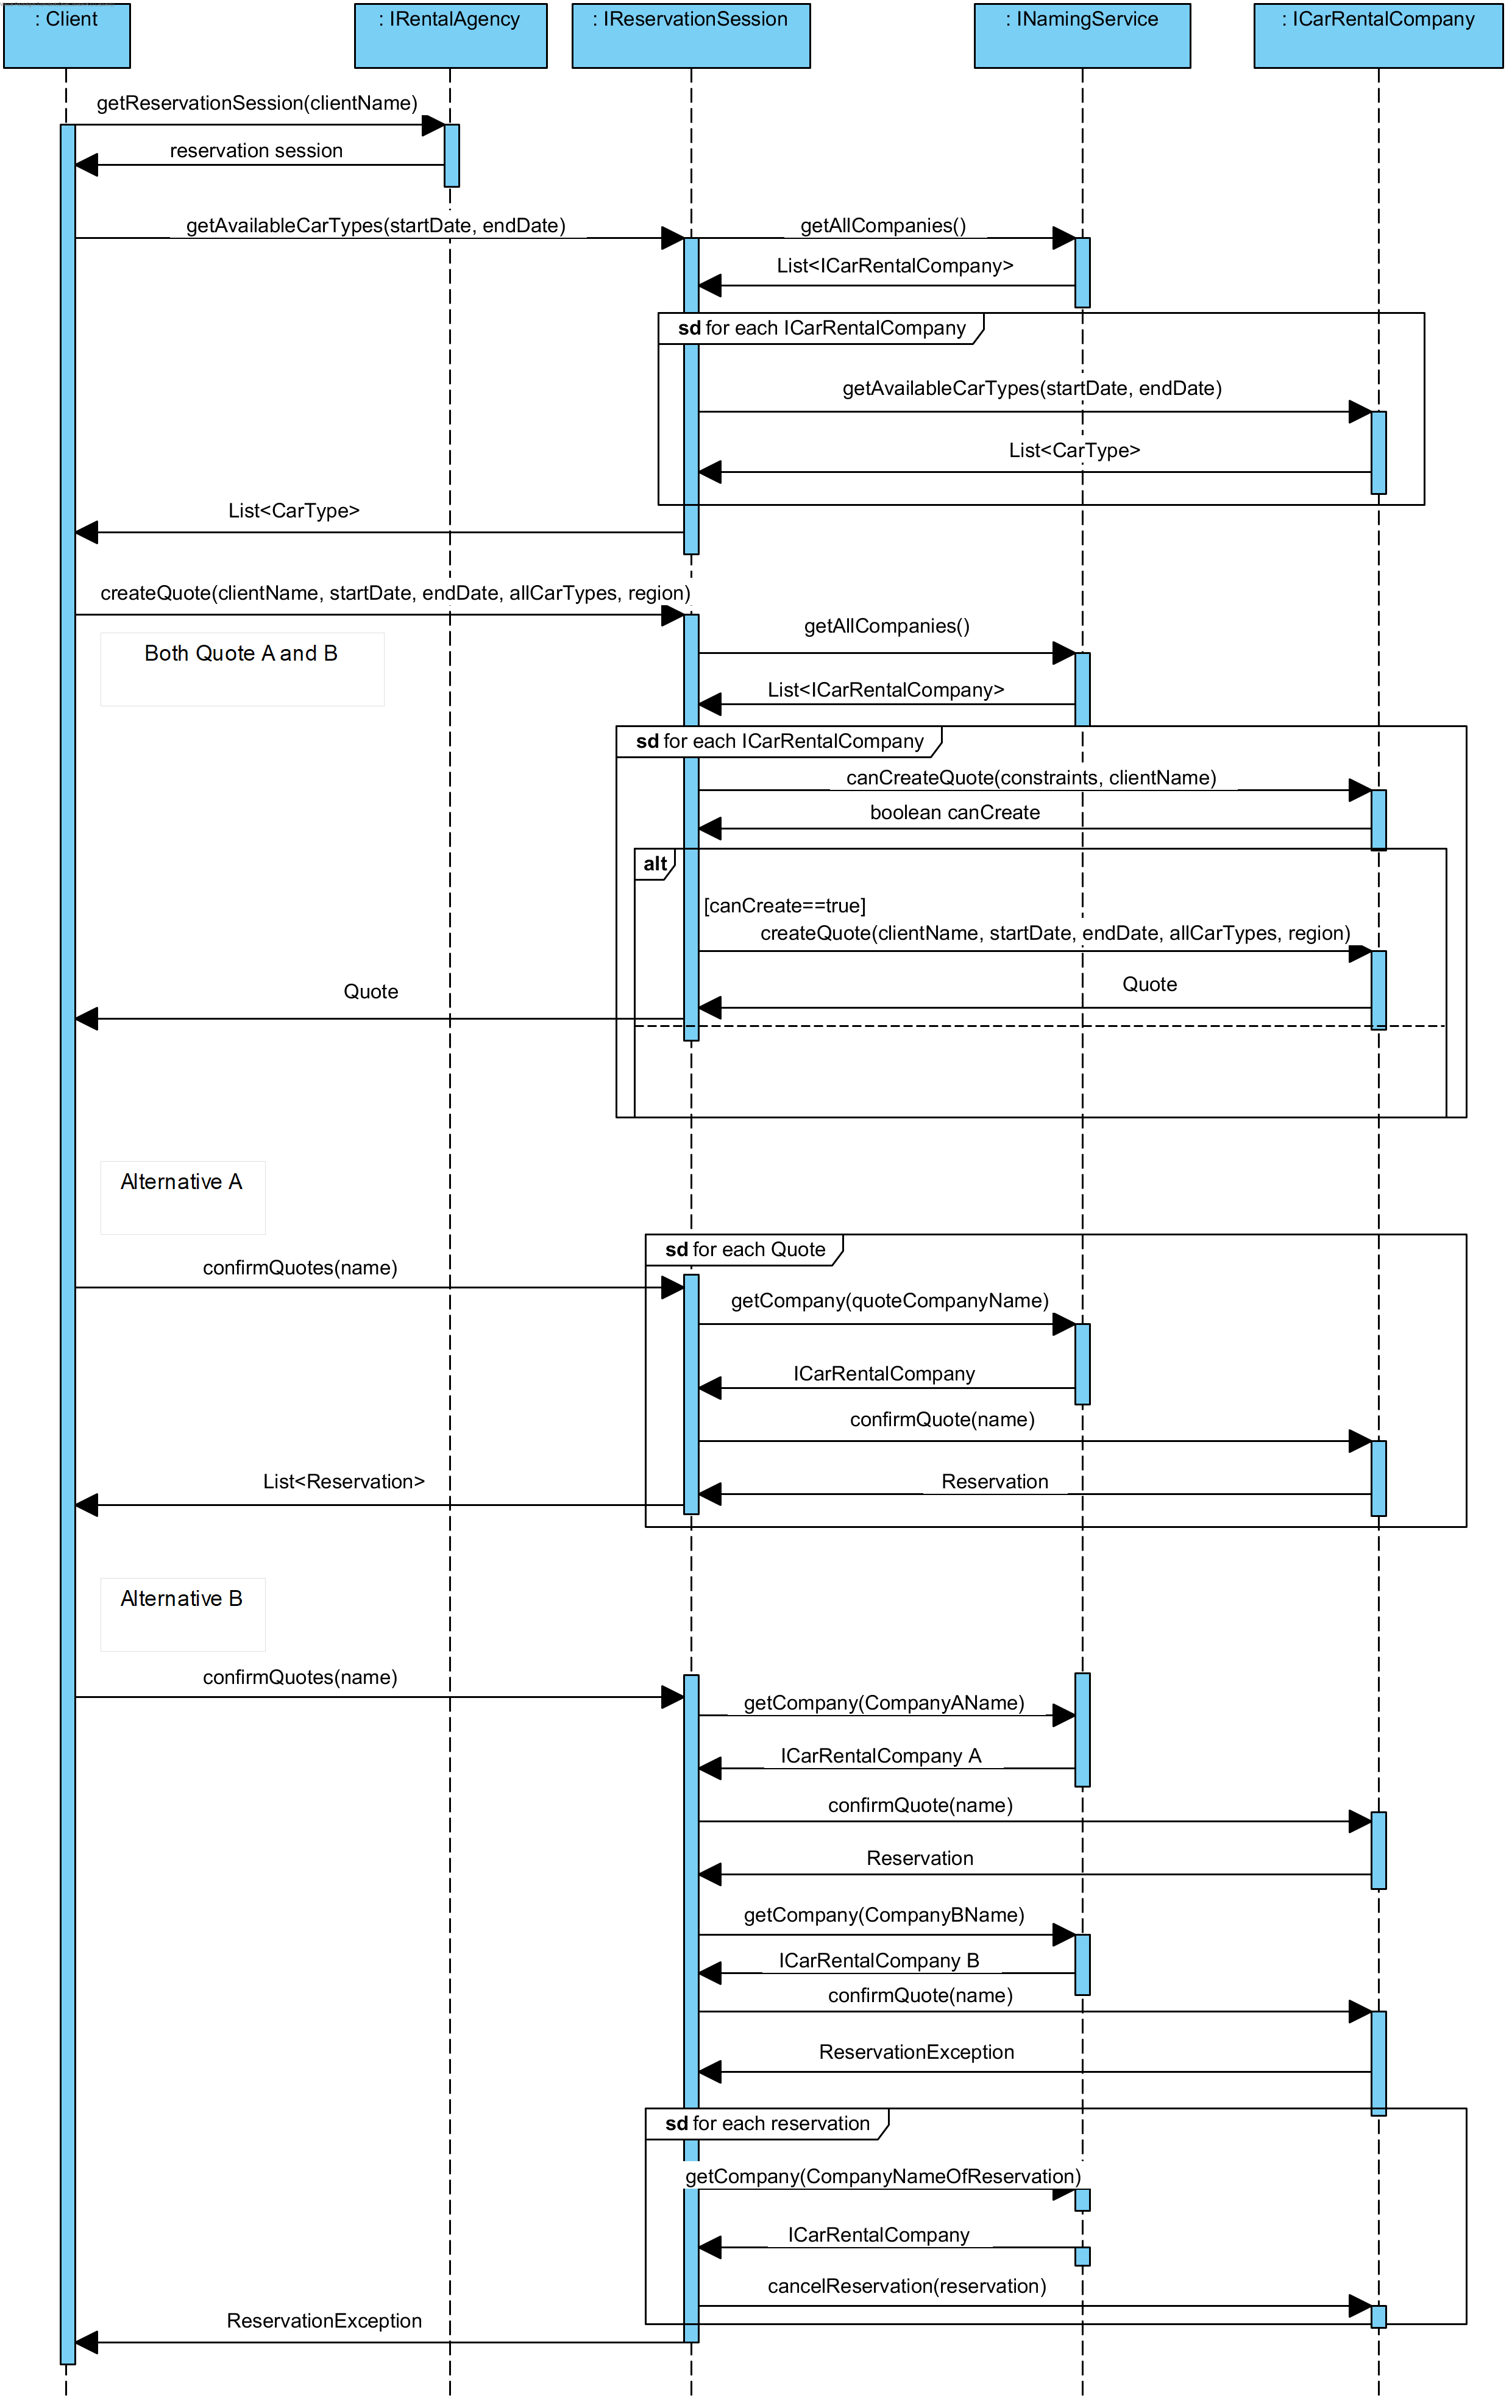
\includegraphics[width=\linewidth]{sequence_diagram.png}
  \caption{Sequence diagram}
  \label{fig:sequence_diagram}
\end{figure}
\begin{figure}[ht]
  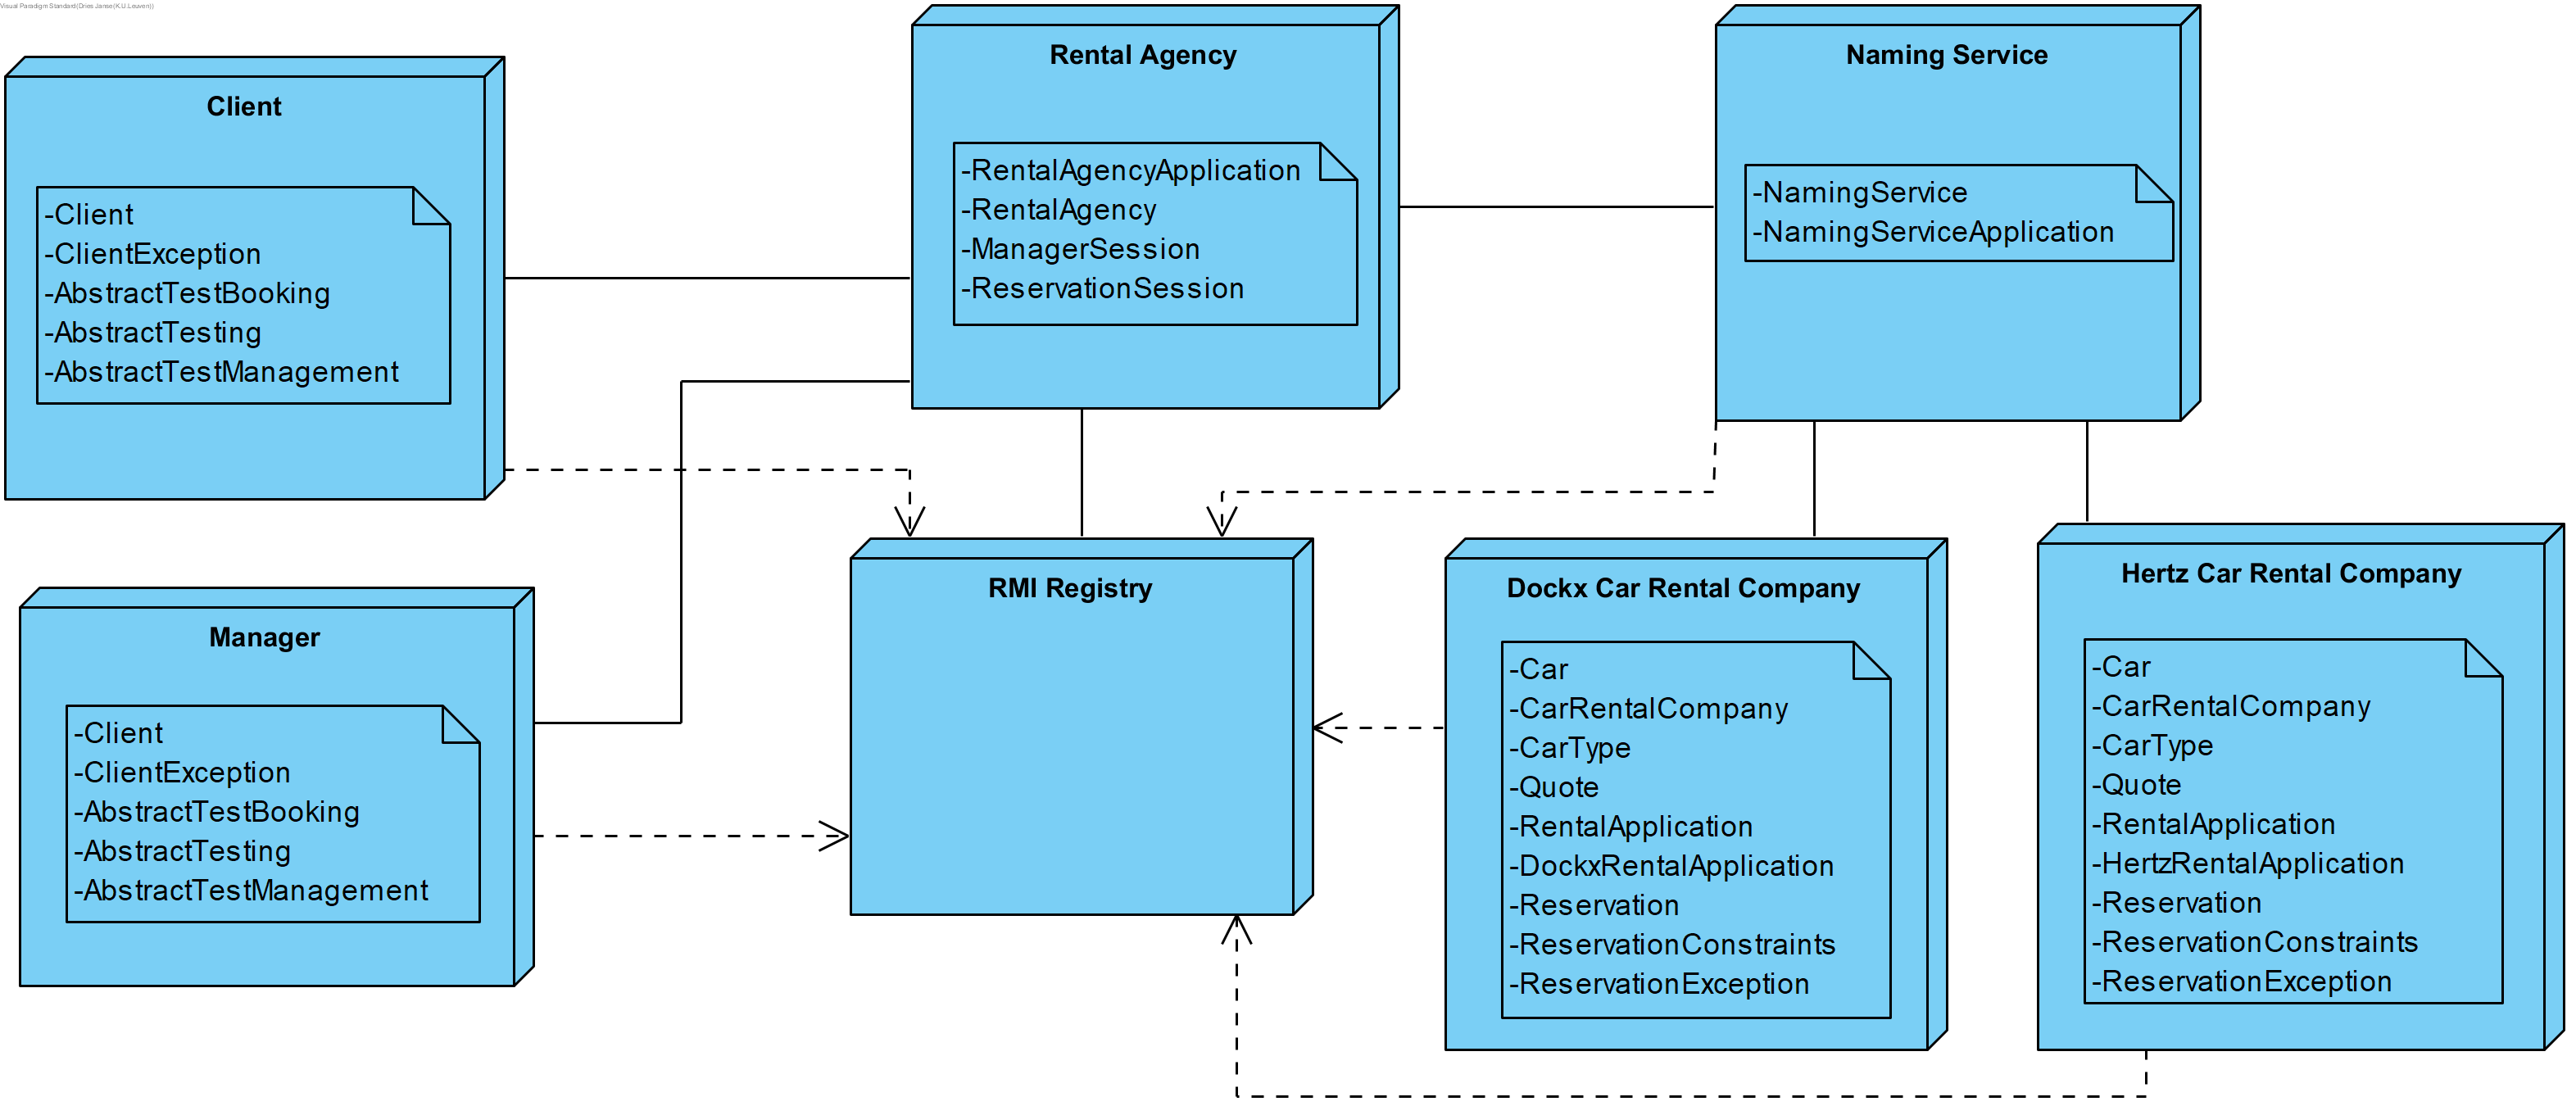
\includegraphics[width=\linewidth]{deployment_diagram.png}
  \caption{Deployment diagram}
  \label{fig:deployment_diagram}
\end{figure}
	% You can include diagrams here.
	
\end{document}